\section{Methods}
\label{sec:ral24_methods}

As this work does not alter the fundamental principles of
\ac{fabrics}, this section focuses on the integration of
three different implicit environment representations into
the framework. In the process, we lay out the necessary
concepts required for the representations, and provide the
tools to combine them with \ac{fabrics}.

\begin{figure}
  \centering
  \input{src/24-spahn-ral/img/methods/inkscape/composition_tex.pdf_tex}
  \caption{Composition of symbolic \ac{fabrics} and runtime loop.\MS{Still to be
  improved.}}
  \label{fig:composition_symbolic_fabrics}
\end{figure}

\subsection{Signed Distance Fields}
\label{sub:signed_distance_fields}

In unknown environments, collision avoidance can be realized using \ac{sdf}.
In this approach, the environment is discretized into a grid and a distance to
the closest obstacle of the environment is assigned to each voxel in the grid.
In this work, we are addressing dynamic environments, so the \ac{sdf} changes
over time, see \cref{fig:sdf} for a two-dimensional example.
%
\begin{figure}[ht]
  \centering
  \begin{subfigure}{0.25\linewidth}
    \centering
    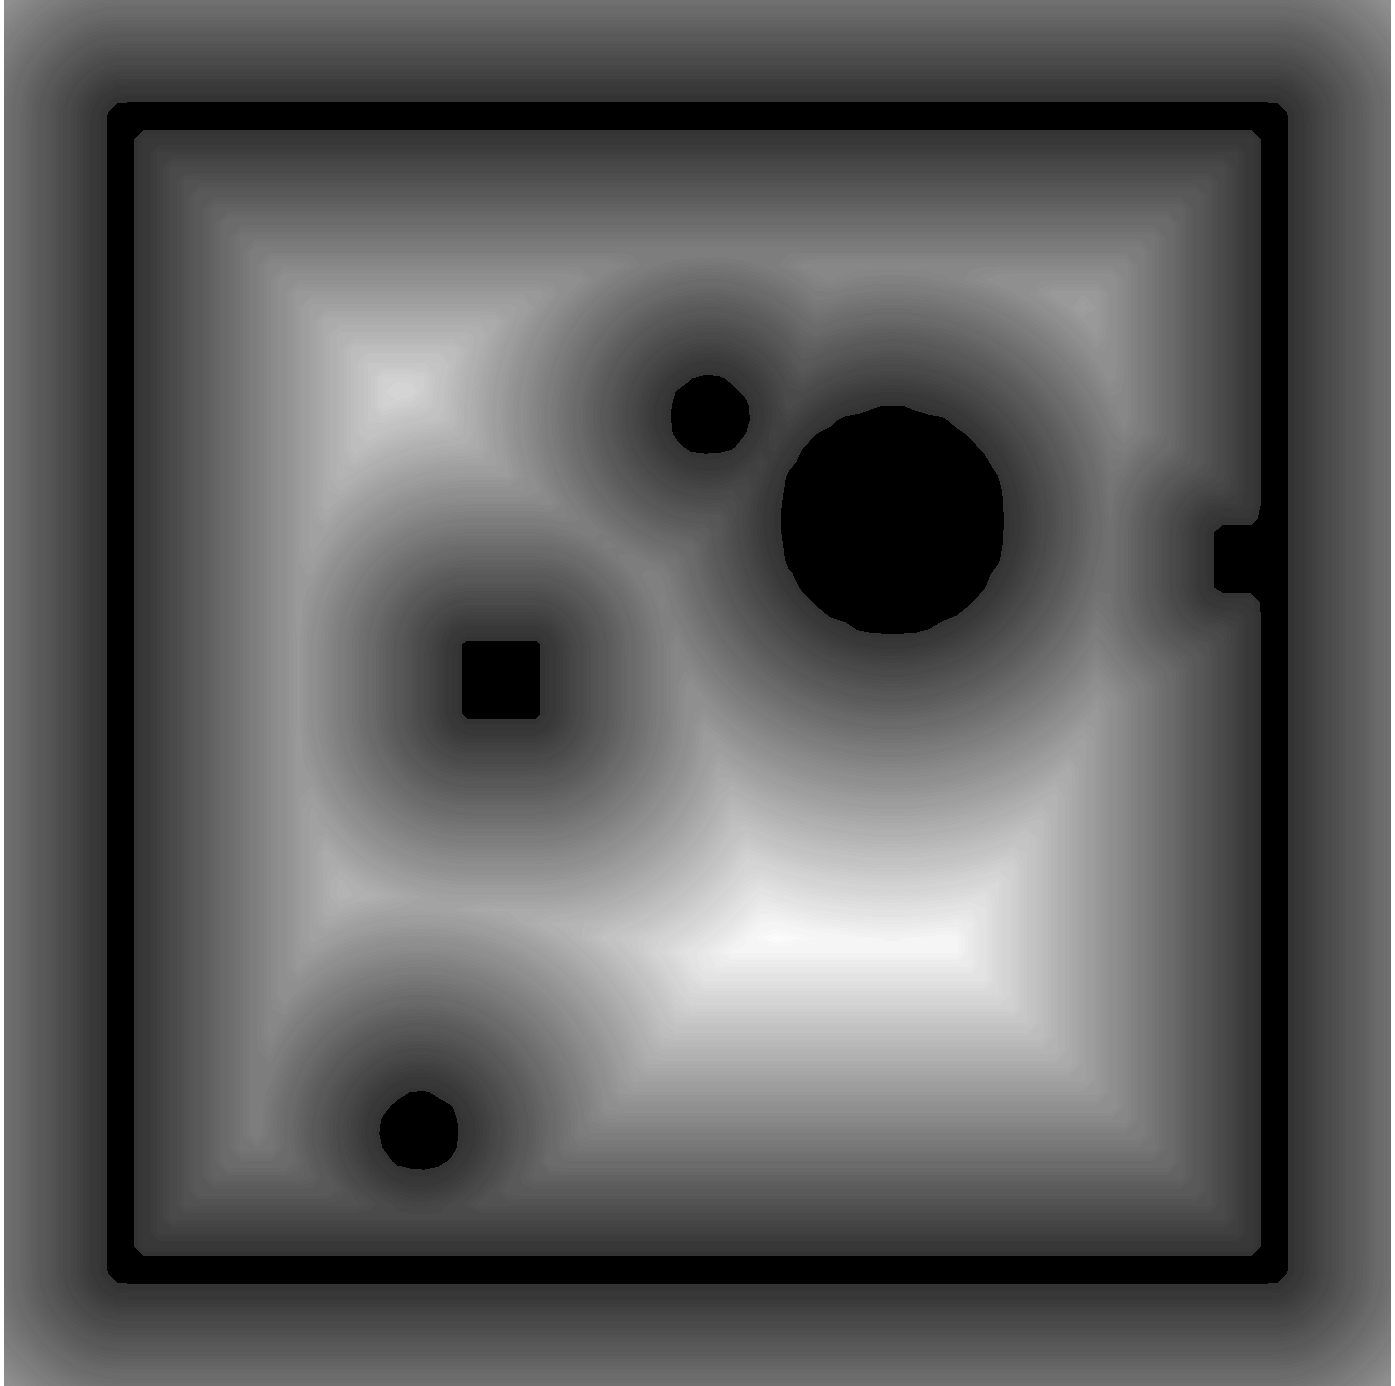
\includegraphics[width=1.00\textwidth]{methods/sdf_1.png}
    \caption{}%
  \end{subfigure}%
  \begin{subfigure}{0.25\linewidth}
    \centering
    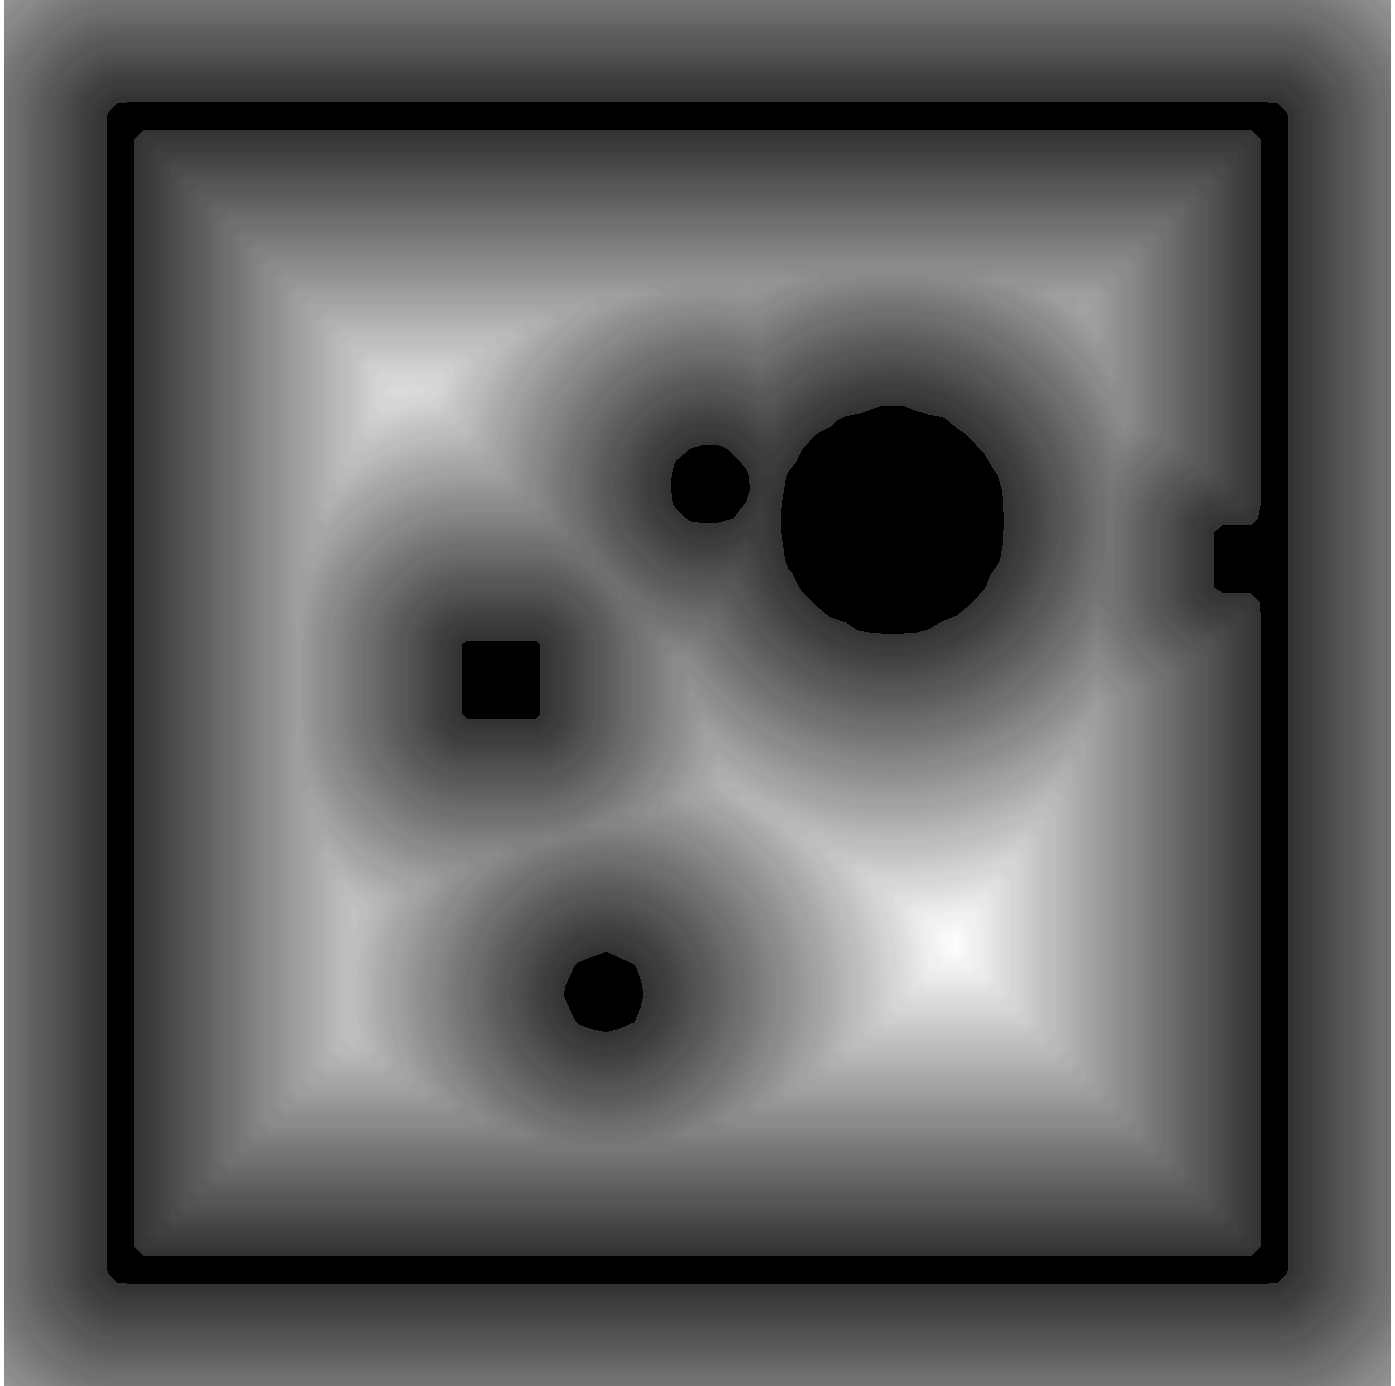
\includegraphics[width=1.00\textwidth]{methods/sdf_2.png}
    \caption{}
  \end{subfigure}%
  \begin{subfigure}{0.25\linewidth}
    \centering
    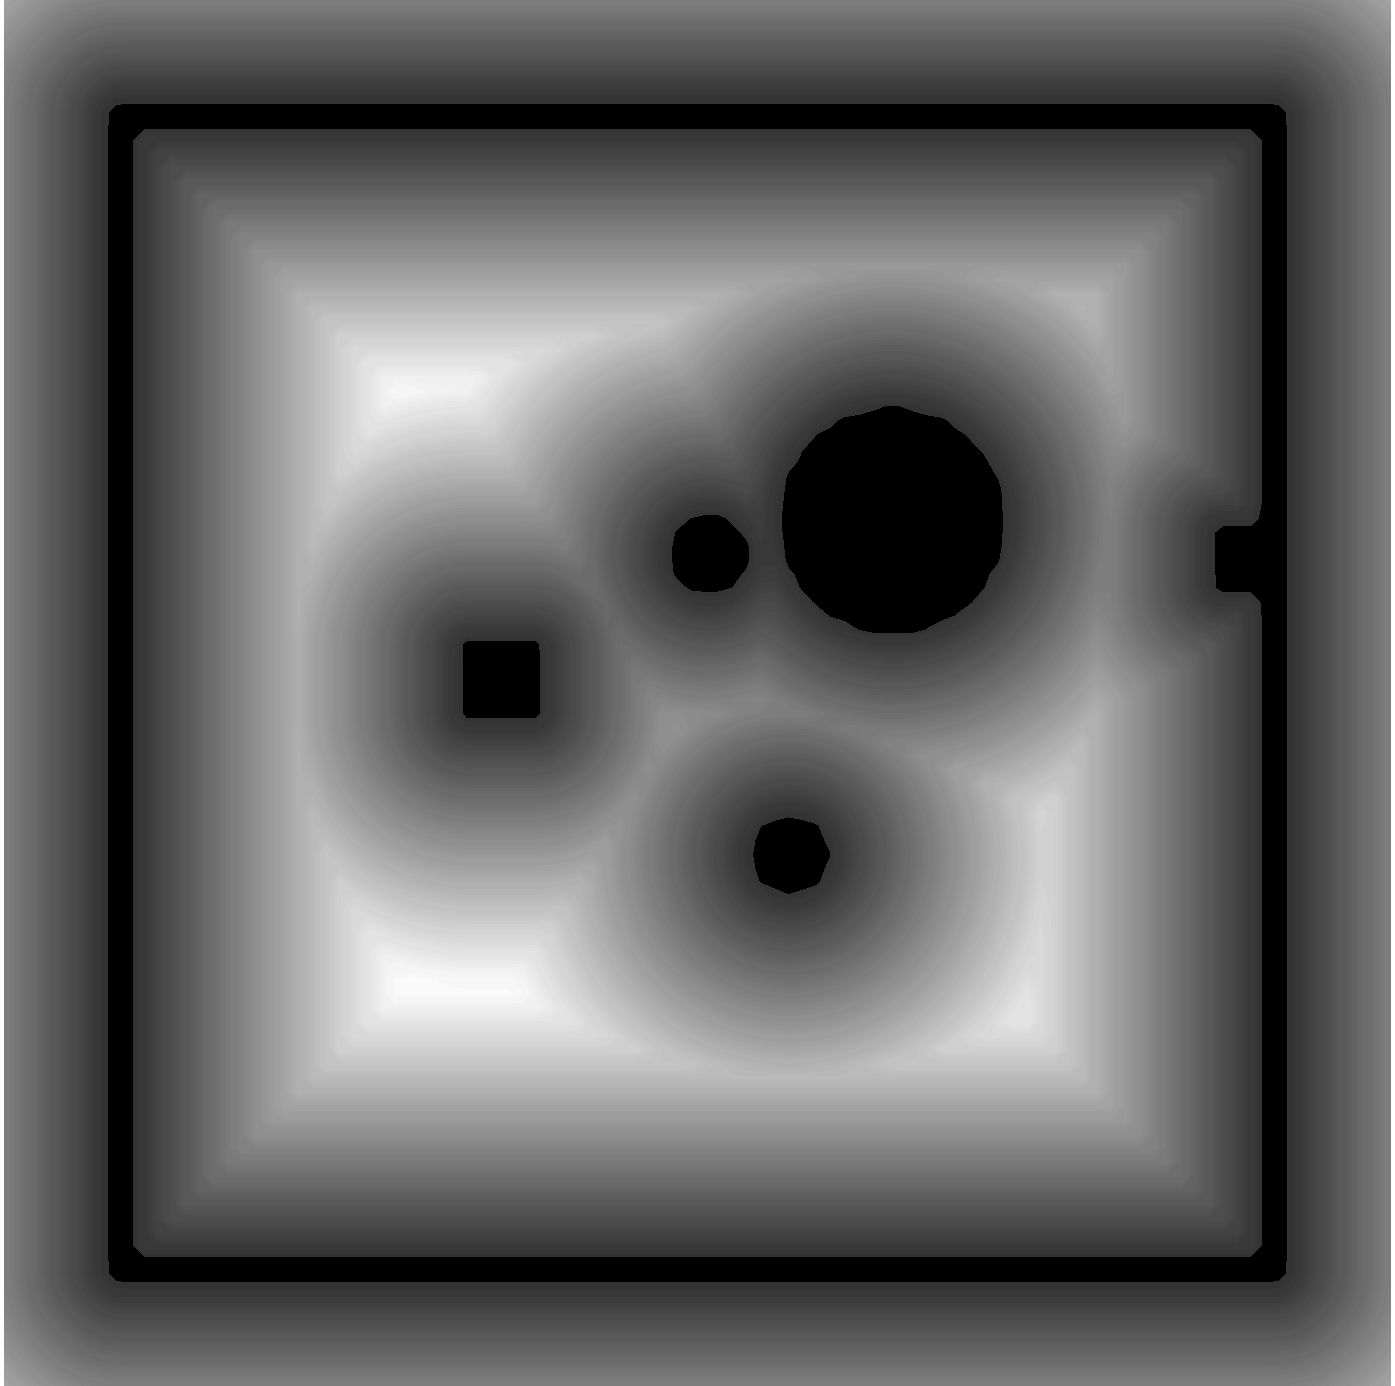
\includegraphics[width=1.00\textwidth]{methods/sdf_3.png}
    \caption{}
  \end{subfigure}%
  \begin{subfigure}{0.25\linewidth}
    \centering
    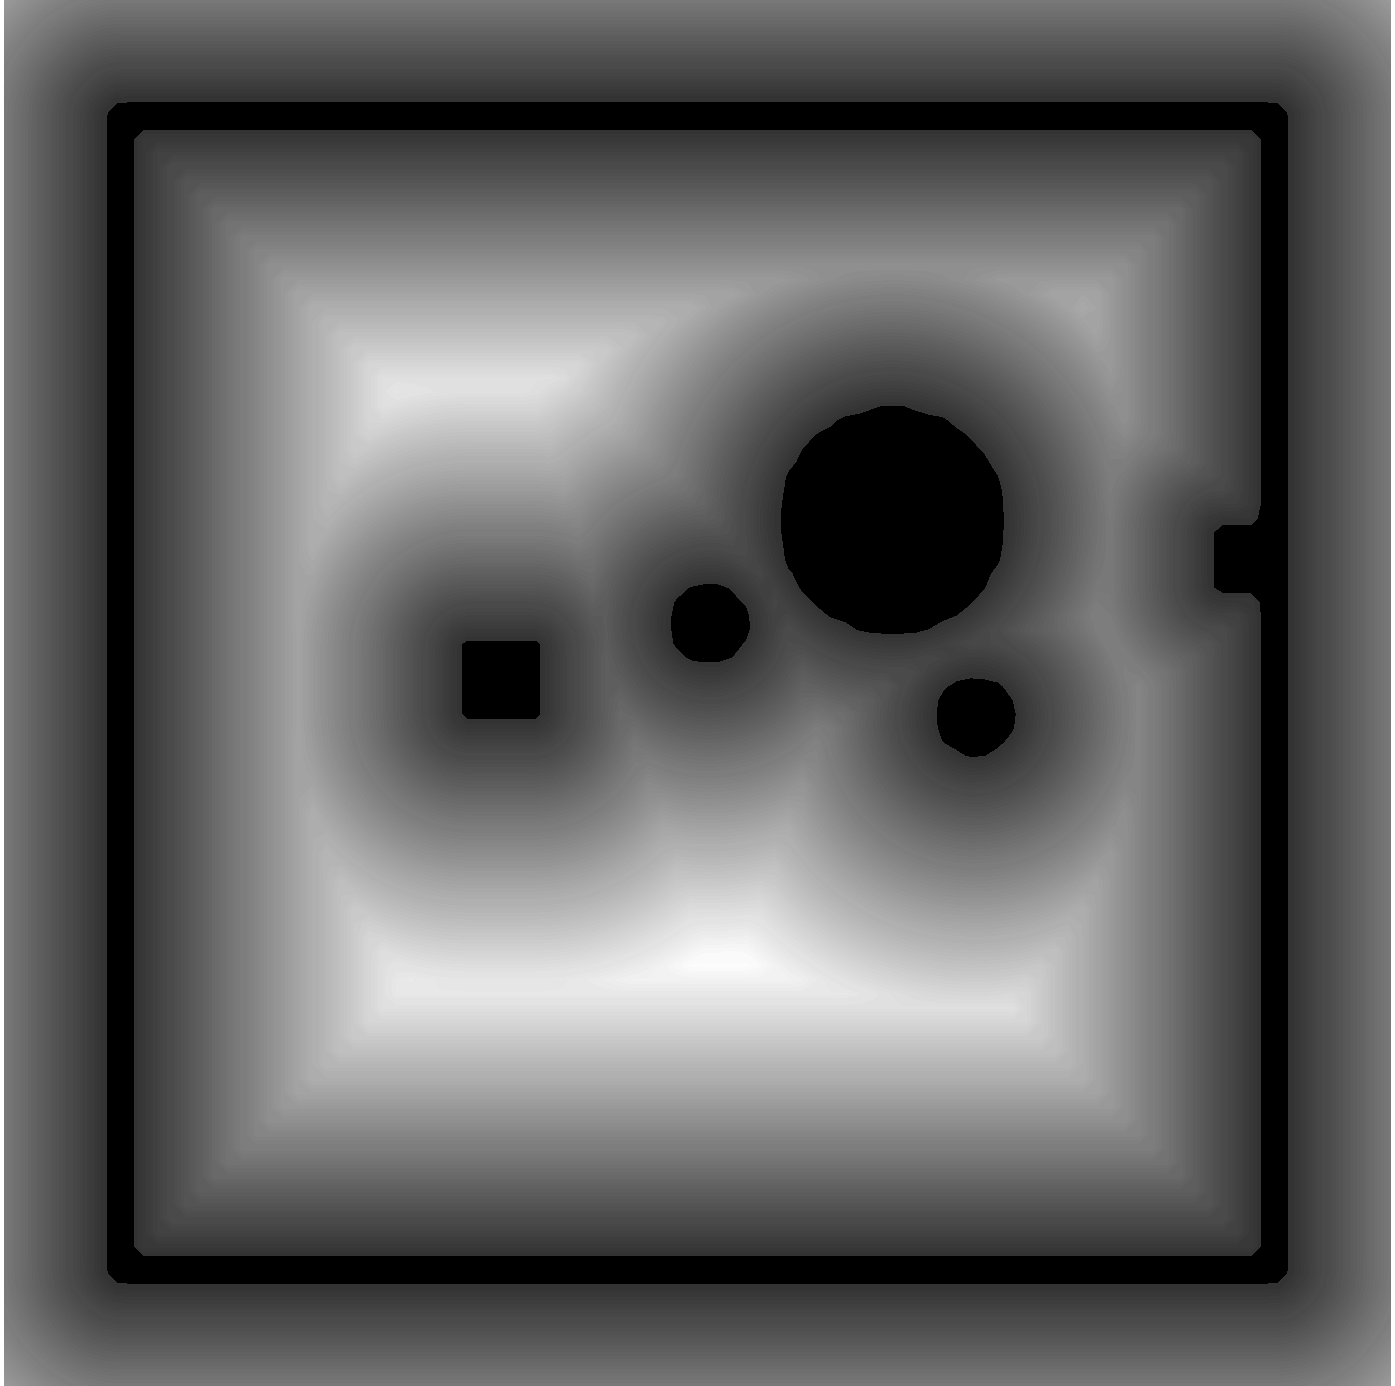
\includegraphics[width=1.00\textwidth]{methods/sdf_4.png}
    \caption{}
  \end{subfigure}
  \caption{Changing Signed Distance Field in 2D.
  }%
  \label{fig:sdf}
\end{figure}

Collision avoidance in the context of \ac{fabrics} is based on
individual task manifolds for each collision obstacle. The geometry and the 
weighing Finsler energy are defined in the correpsonding task manifold \X{}.
To combine those tasks the geometries and the energies are pulled back into the
root space, usually defined as the configuration space \Q{}. According 
to \cref{eq:pullback}, this requires the computation of the gradient \J{}.
When the environment is represented as a \ac{sdf}, the gradient cannot be
computed analytically, as it is possible for simple geometric shapes in
\cite{Ratliff2021,Spahn2023}. To overcome this limitation, we propose to
use the numerical gradient as an approximation instead.
The \ac{sdf} is evaluated based on the forward kinematics of the collision link,
so $\map_{sdf}(\fk)$ is a function of \q{}.
As $\der{\q}{\map_{sdf}}$ is not analytically accessible due to the numerical
nature of signed distance fields, we apply the chain rule to obtain
\[
  \derf{\q}{\map_{sdf}} = \derf{\fk}{\map_{sdf}}\derf{\q}{\fk}.
\]
The second term $\der{\q}{\fk}$ is the gradient of the forward
kinematics, which can be computed analytically. The first part is the gradient
of the \ac{sdf} which can be
approximated using finite differences:
\[
  \left(\derf{\fk}{\map_{sdf}}\right)_i \approx 
  \frac{\map_{sdf}(\fk + \Delta_i e_i) - \map_{sdf}(\fk - \Delta_i e_i)}{2 \Delta_i},
\]
where $\Delta$ is the resolution in the $i$-th dimension. For optimization
\ac{fabrics}, the gradient and the value of the \ac{sdf} must be computed externally
at each time step, while the analytical compenent is stored internally. Similar
to \cite{Ratliff2021}, we omit the curvature term \Jdot{} in the pull-back
operation.
\MS{Can we think about a figure here?}

When working with multi-link robots, such as manipulators, different manifolds
are created for the different collision links. Note, that the same signed
distance field can be used and does not require extra computation.

\subsection{Free Space Decomposition}
\label{sub:Free Space Decomposition}

\begin{figure}[ht]
  \centering
  \begin{subfigure}{0.33\linewidth}
    \centering
    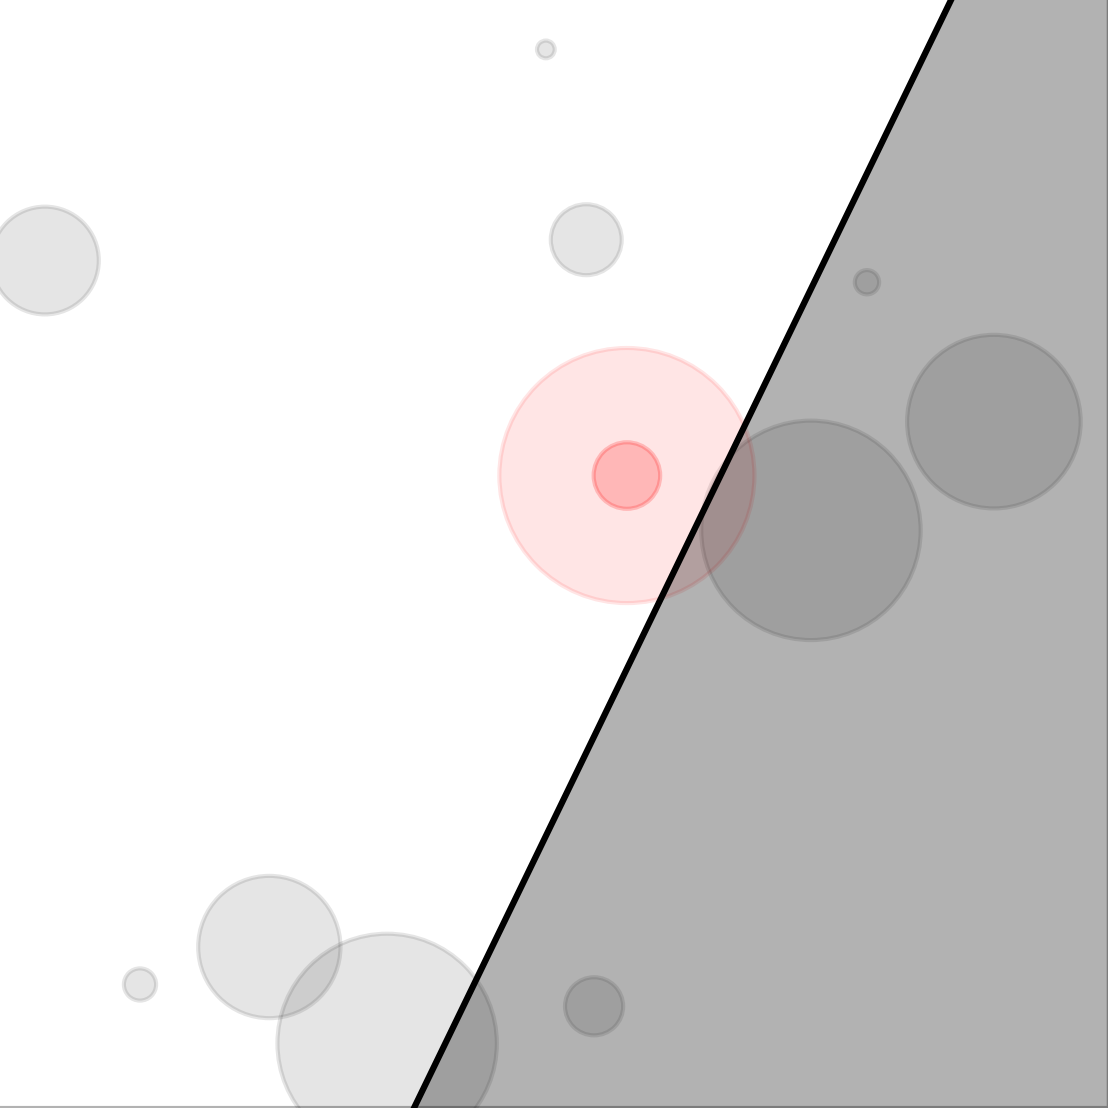
\includegraphics[width=.95\textwidth]{methods/fsd_plot_0.png}
    \caption{}%
  \end{subfigure}%
  \begin{subfigure}{0.33\linewidth}
    \centering
    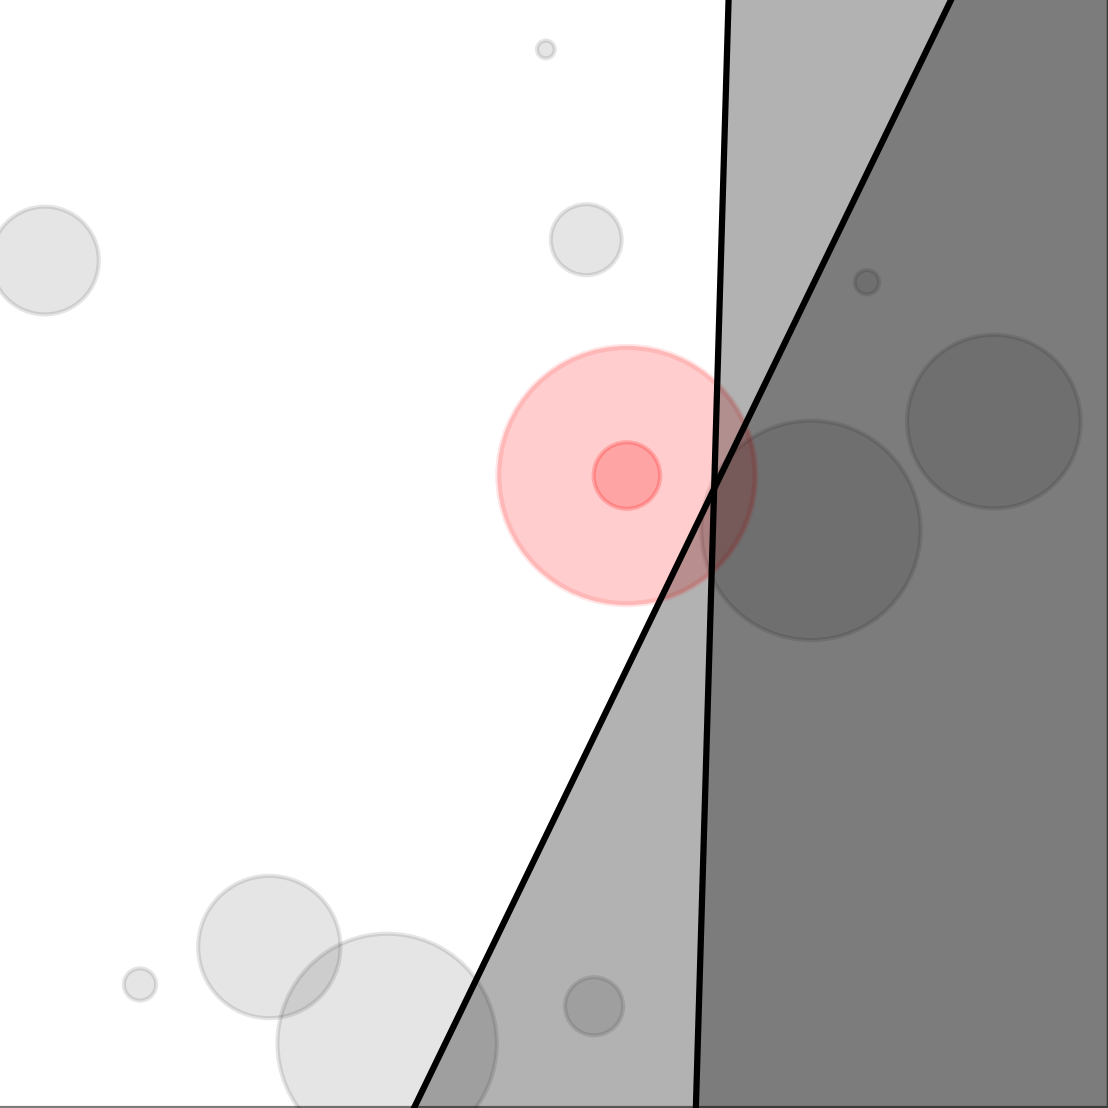
\includegraphics[width=.95\textwidth]{methods/fsd_plot_1.png}
    \caption{}
  \end{subfigure}%
  \begin{subfigure}{0.33\linewidth}
    \centering
    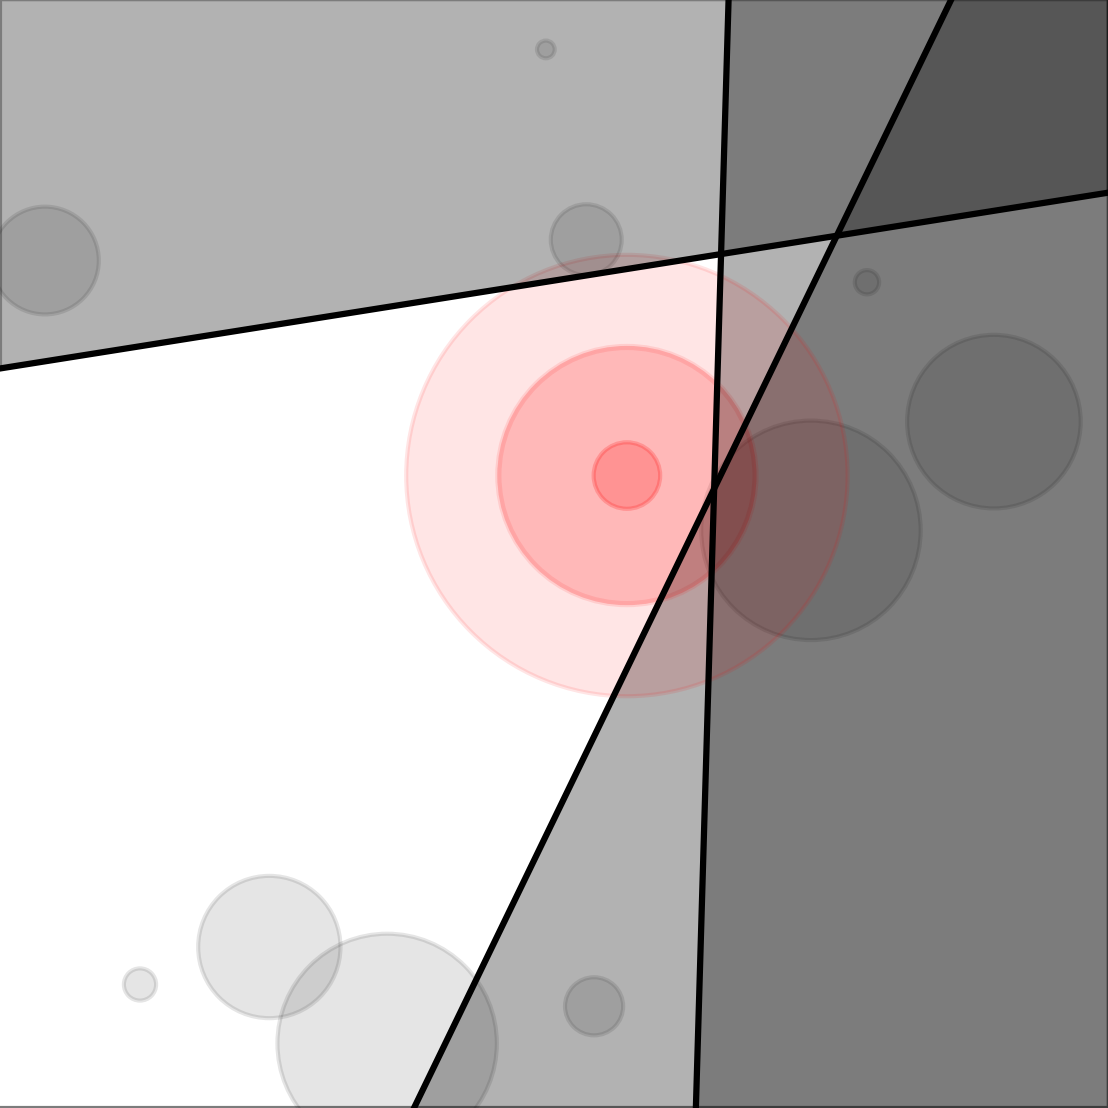
\includegraphics[width=.95\textwidth]{methods/fsd_plot_2.png}
    \caption{}
  \end{subfigure}
  \begin{subfigure}{0.33\linewidth}
    \centering
    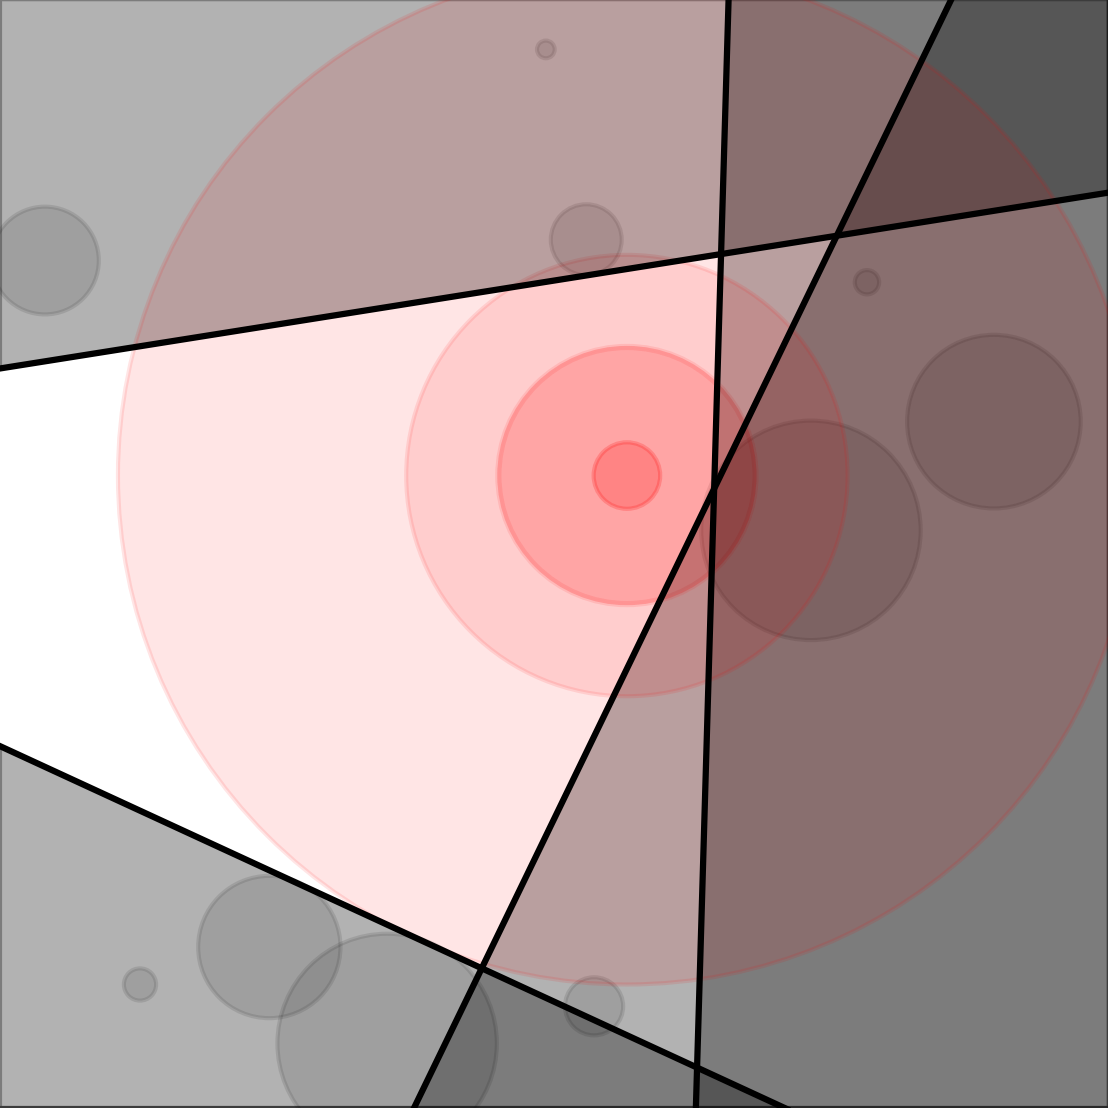
\includegraphics[width=.95\textwidth]{methods/fsd_plot_3.png}
    \caption{}
  \end{subfigure}%
  \begin{subfigure}{0.33\linewidth}
    \centering
    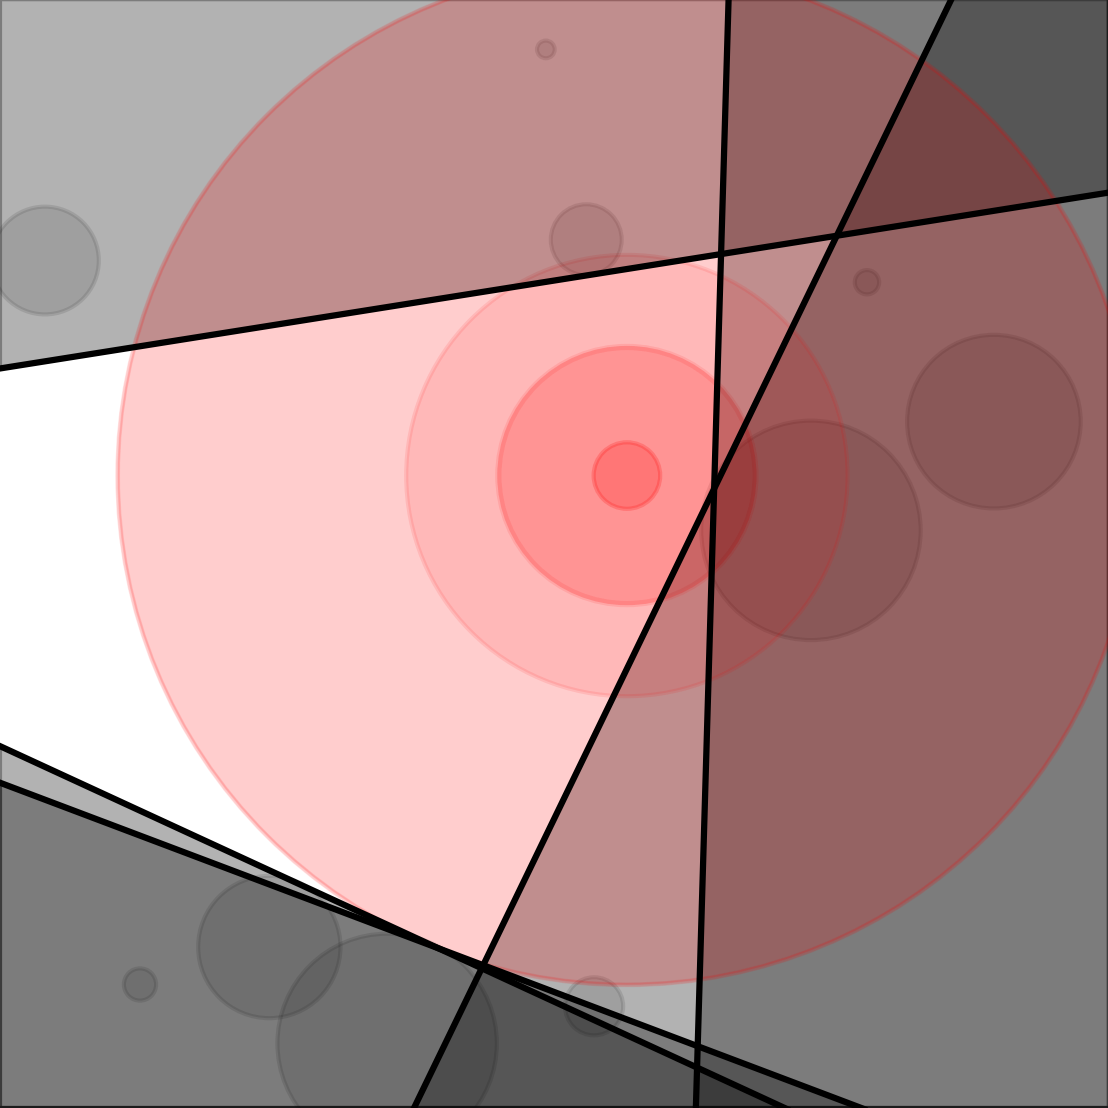
\includegraphics[width=.95\textwidth]{methods/fsd_plot_4.png}
    \caption{}
  \end{subfigure}%
  \begin{subfigure}{0.33\linewidth}
    \centering
    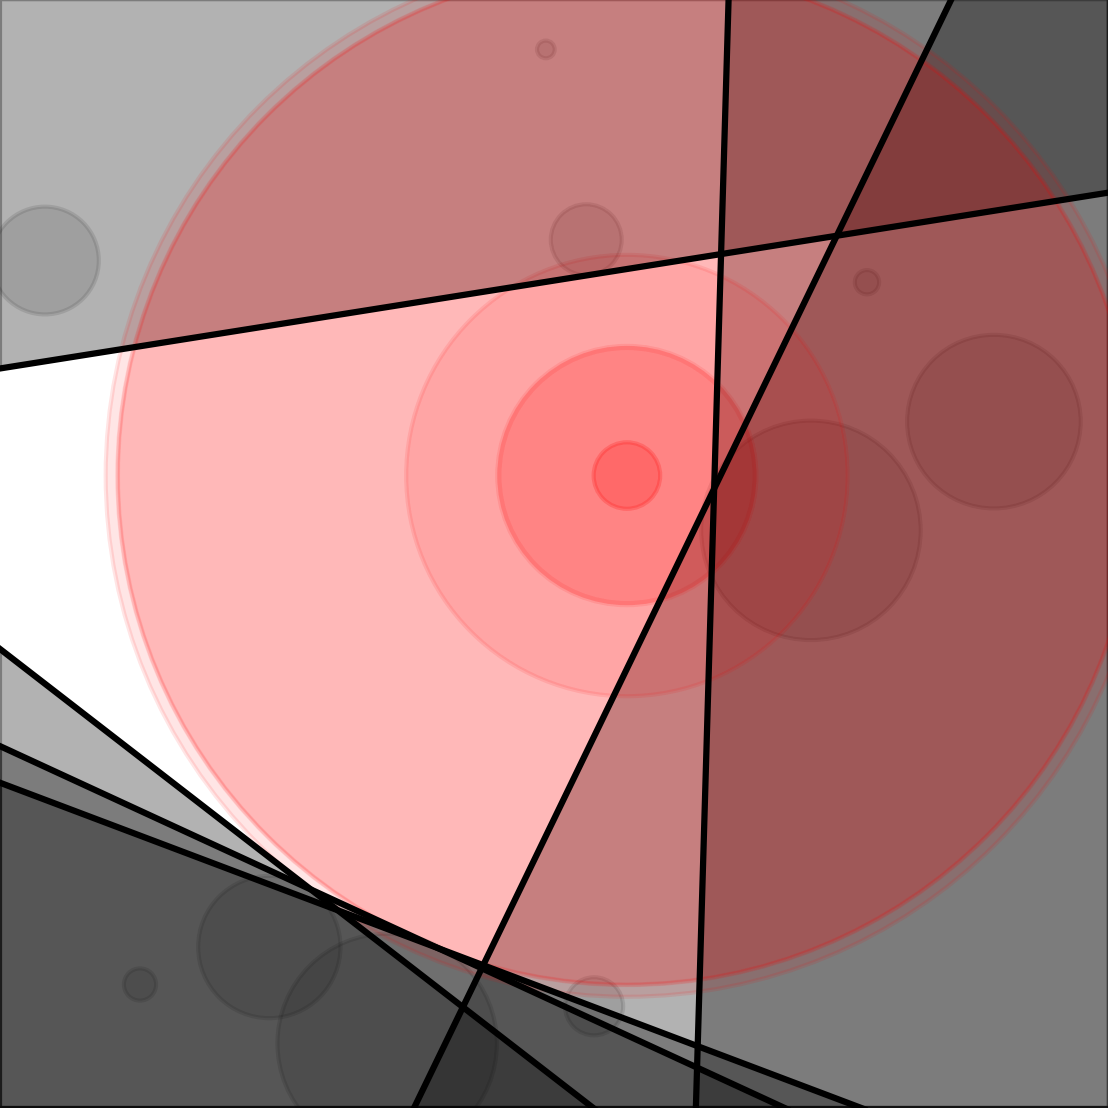
\includegraphics[width=.95\textwidth]{methods/fsd_plot_5.png}
    \caption{}
  \end{subfigure}%
  \caption{Iterative \acl{fsd} in 2D. The \seed{} is shown in red, obstacles in
    light gray, each \plane{} by black plane and the block workspace is shaded
    in gray. The resulting \acs{fsd} is the remaining white space.
  }%
  \label{fig:fsd}
\end{figure}

When posing trajectory generation as a constrained optimization problem, for
examplel in the form of \ac{mpc}, constraints for collision avoidance can be of
any form. Very popular in recent literature
\cite{Tordesillas2019,Liu2017a,Spahn2021} is to decompose the environment with
all its obstacles, including dynamic obstacles, into a \ac{fsd} Then, the
workspace in the constrained optimization is reduced to free space. 

The method used in this work is inspired by \cite{Liu2017a}. We define the
\seed{} for the \ac{fsd} as the \fk{} of the collision link in question. Then,
\pointcloud{} is sorted according to the euclidean distance to the \seed{}.
Starting with the closest point, a plane \plane{} defined by $\np = \point -
\seed$ and $\cp = \point$ for every $\point \in \pointcloud$. To further
speedup the process, every \point{} in \pointcloud{} that is `behind' an
existing \plane{} is removed from the \pointcloud{}. The method results in set
of $\set_{\textrm{planes}} = \{\plane_i, i\in[0,n]\}$ representing the free
space around \seed{}. The algorithm is visualized in \cref{fig:fsd} for a 2D
case.
\MS{Think about pseudo code.}

In this work, we propose a method to integrate free space
decomposition into the framework of optimization \ac{fabrics}. Specifically, we
define a differentiable mapping from configuration space \Q{} to the distance
manifold between robot and each constrained plane \plane{}. Given the forward
kinematics of a collision link on the robot by \fk{} and the radius of the
collision link, the distance to the plane \plane{} defined by its normal
\np{} and the constart \cp{}, the distance is computed as:
\begin{equation}
  \map({\plane,\fk,\rl}) = \frac{\np^T\fk + \cp}{\norm{\np}} - \rl
  \label{eq:point_plane_distance}.
\end{equation}
In contrast to signed distance fields, the gradients, \J{} and \Jdot{}, can be
computed analytically as a function of \q{}, \np{} and \cp{}.



\subsection{Raw Sensor Integration}
\label{sub:raw_sensor_integration}


When trajectory generation is formulated as receeding horizon optimization, such
that the optimization problem is solved iteratively in every time step, the
amount of constraints must be limited so that the computational costs stay
within boundaries. Thus, raw sensor data, such as lidar data, point clouds or 
occupancy maps, must be processed to limit the number of constraints (or cost
terms). On the other side, as optimization \ac{fabrics} can be formulated entirely
symbolically, the computational costs can be reduced drastically
\cite{Spahn2023}. This allows to reduce the amount of preprocessing,
limiting the amount of uncertainty and room for error in this step. Here, we
explain how raw lidar sensor data can be used with optimization \ac{fabrics}.
The same approach can be used to directly integrate pointclouds or occupancy
grids.

We assume that a sensor outputs a set of $n_{\textrm{points}}$
points \pointcloud{} in the robot`s workspace. For example, a two-dimensional
lidar sensor produces $n_{\textrm{points}}=resolution_{lidar}$ points
$\pointcloud_{\textrm{lidar}}$. We integrate this data directly into
optimization \ac{fabrics} by placing a virtual, spherical obstacle at each $\point
\in \pointcloud$. The radius of these obstacles must be chosen to reflect the
resolution of the point cloud.




